\section{Client}
How the client is implemented are similar on what we describe in Table \ref{tab:tools-table} despite that the database has been substituted with a simple file with aim to simulate a device memory.

The client wants to simulate as much as possible a real temperature sensor because we don't have the sensor and any kind of board available.

Another fact that it isn't clear from the original paper, is the concept of \textbf{session}. We assume that the session is defined by the IoT device because is the component that starts all the authentication and then, after the authentication process, sends its data for a certain amount of time before closing the session and updates its secure vault.
After closing the session the device waits a couple of seconds before initiate new session sending its device and session id.

\begin{lstlisting}[language=Python, basicstyle=\tiny, label={lst:client}, caption=Client logic]
op_res = helper.set_vault()

if not op_res.startswith("FAILED"):
     while True:
        buffer: str = ""
        # Create a TCP socket
        sock = socket.socket(socket.AF_INET, 
                             socket.SOCK_STREAM)
        sock.settimeout(TIMEOUT)

        sock.connect((HOST, PORT))
        sock.settimeout(TIMEOUT)

        try:
            # STEP 1: sends M1
            
            sock.sendall(helper.create_m1(DEVICE_ID, SESSION_ID))

            # STEP 2: receives M2
            m2 = sock.recv(1024)
            m2 = str_to_dict(m2.decode())

            c1, r1 = [i for i in map(int, m2['C1'].split(','))], 
                        m2['r1']

            helper.set_c1(c1)
            helper.set_r1(r1)
            del c1, r1

            # STEP 3: send M3
            sock.sendall(helper.create_m3())

            # STEP 4: receive M4
            m4 = sock.recv(1024)

            # STEP 4-5: verifying server response
            if helper.verify_server_response(m4):
                
                # SENDING DATA until the end of the session
                ...
                
                if not len(buffer) == 0:
                    # STEP 6: update the secure vault
                    helper.update_vault(buffer.encode())

            time.sleep(1)
         except socket.timeout:
            sock.close()
         except ValueError:
            sock.close()
            break
        except OSError:
            break
\end{lstlisting}

\subsection{Sensor implementation}
As mention above we want to get a realistic sensor simulation. To do so, we image a possible scenario where we put a temperature sensor indoor without any external intervention (for instance, opening a door or window). To reach our objective, we decided to sample the temperature from a normal distribution centered on 18°C with a standard deviation of 1 because gives us a more realistic temperature variation for an indoor environment (see Figure \ref{fig:temp-distribution}).

\begin{figure}[h]
    \centering
    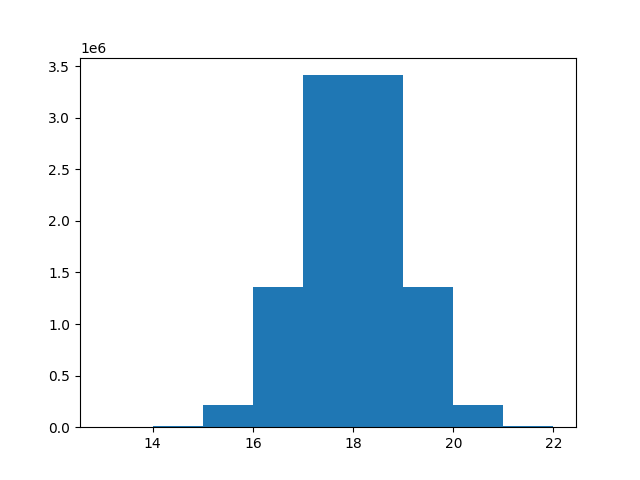
\includegraphics[width=.48\textwidth]{imgs/temp-distribution.png}
    \caption{Temperature distribution}
    \label{fig:temp-distribution}
\end{figure}
